\documentclass[12pt]{article}

% Specify how big is going to be the paper margins.
\usepackage[a4paper, margin=1in]{geometry}

% amsmath: Add useful commans like aligh and gather.
% amsfonts: Add useful fonts like \mathbb{R}.
% amssymb: Add useful symbles like \therefore (needs amsfonts to work).
\usepackage{amsmath, amsfonts, amssymb}

% Makes the use of colors possible.
\usepackage{xcolor}

\definecolor{color1}{HTML}{084a8c}
\definecolor{color2}{HTML}{487fb7}
\definecolor{color3}{HTML}{95b7da}
\definecolor{color4}{HTML}{c9daea}

% Add Latin Modern Fonts like Sans-serif and Roman.
\usepackage{lmodern}

% Makes header and footer configurable.
\usepackage{fancyhdr}

% Makes the use of colored and configured tables possible
\usepackage{tcolorbox}

% Add commands to specify theorems like \newtheorem{x}{y}.
\usepackage{amsthm}

% Enables enumeration of items.
\usepackage{enumitem}

% Enables adding images.
\usepackage{graphicx}

% Enables cool hyper references.
\usepackage[colorlinks=true, linkcolor=color2, urlcolor=color2, citecolor=color2]{hyperref}

\title{\sffamily\bfseries{Soluções Jacob Palis 2024 N2}}
\author{Samuel de Araújo Brandão}
\date{4 de Setembro de 2025}

\pagestyle{fancy}
\fancyhf{}

\fancyhead[L]{\sffamily\bfseries{Soluções Jacob Palis 2024 N2}}
\fancyhead[R]{\textcolor{color2}{Samuel Brandão}, 4 de Setembro de 2025}
\fancyfoot[C]{\thepage}
\setlength{\headheight}{14.5pt}

\tcbset{
  statementbox/.style = {
    enhanced,
    width=\textwidth,

    title={Enunciado},
    titlefilled,
    fonttitle=\sffamily\bfseries,
    coltitle=color4
    colbacktitle=color1,

    colback=white,
    colframe=color1,
    boxrule=1pt,
    arc=2mm,
    boxsep=2pt,
  }
}

\tcbset{
  theorembox/.style = {
    enhanced,
    width=\textwidth,

    colback=white,
    colframe=color1,
    boxrule=1pt,
    arc=2mm,
    boxsep=2pt
  }
}

\tcbset{
  lemmabox/.style = {
    enhanced,
    width=\textwidth,

    colback=white,
    colframe=color2,
    boxrule=1pt,
    arc=2mm,
    boxsep=2pt
  }
}

\renewcommand*\contentsname{\textsf{Conteúdos}}
\newcommand{\kb}[1]{\left\lfloor #1 \right\rfloor}

\begin{document}
  \maketitle
  Uma coleção de soluções para a \textbf{Jacob Palis 2024 Nível 2}, inspirada no estilo de Evan Chen.
  Pode-se encontrar todos os problemas e respostas oficiais 
  \textbf{\href{https://www.obm.org.br/content/uploads/2024/06/jacob_palis_2024_provas_e_solucoes.pdf}{aqui}}.

  Todas as soluções foram inteiramente escritas por mim, enquanto me preparava para a
  International Mathematical Olympiad (IMO).

  Caso encontre algum erro ou tiver sugestões ou comentários, sinta-se a vontade 
  para entrar em contato!

  \tableofcontents

  \clearpage

  \section{\textsf{Problemas}}
    \subsection{Testes}
      \begin{enumerate}[label=\textbf{\arabic*.}]
        \item Sejam \(x, y, z, w\) inteiros positivos tais que \(2024 = 2^x \cdot 5^y = 8^z \cdot 25^w\). Qual é o valor de \(x + y + z + w\)?
        \item Lucas estava participando de uma corrida de rua de 21 quilômetros e monitorava o tempo médio por quilômetro. Ao final do quilômetro
          14, seu ritmo médio era de 6 minutos e 42 segundos por quilômetro. Nos últimos 7 quilômetros, o ritmo caiu, e seu tempo médio no total
          da prova tornou-se 6 minutos e 50 segundos por quilômetro. Qual foi o tempo médio de Lucas nos últimos 7 quilômetros?
        \item Qual o número máximo de meses com 5 quintas-feiras que um ano pode ter?
        \item Quantos triângulos na figura abaixo têm soma de seus números par?
          \begin{figure}[h]
            \centering
            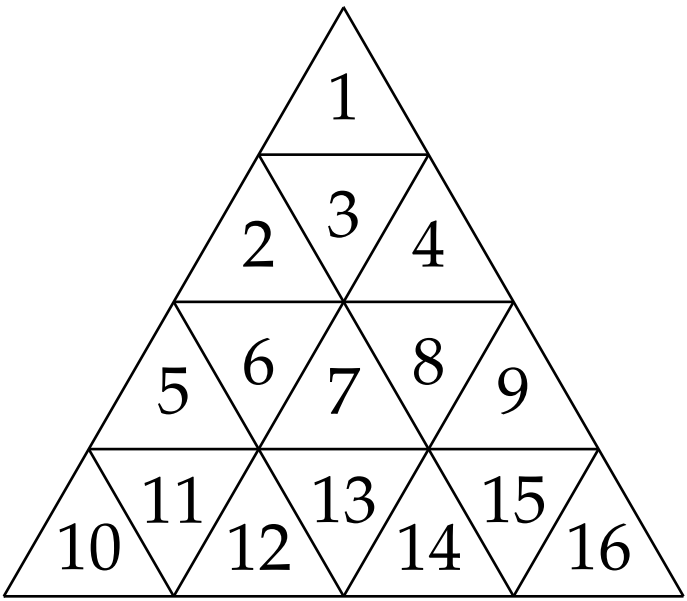
\includegraphics[width=0.3\textwidth]{first.png}
          \end{figure}
        \item Em um retângulo está um pentágono regular, um triângulo equilátero e um quadrado. Os três polígonos compartilham um vértice.
          Os outros dois vértices do triângulo equilátero estão situados, respectivamente, sobre os lados do pentágono e do quadrado. Os outros
          vértices do pentágono e do quadrado estão sobre lados do retângulo. Sabe-se que os lados do pentágono e do quadrado formam ângulos
          iguais \(x\) com lados opostos do retângulo. Qual é o valor de \(x\) em graus?
          \begin{figure}[h]
            \centering
            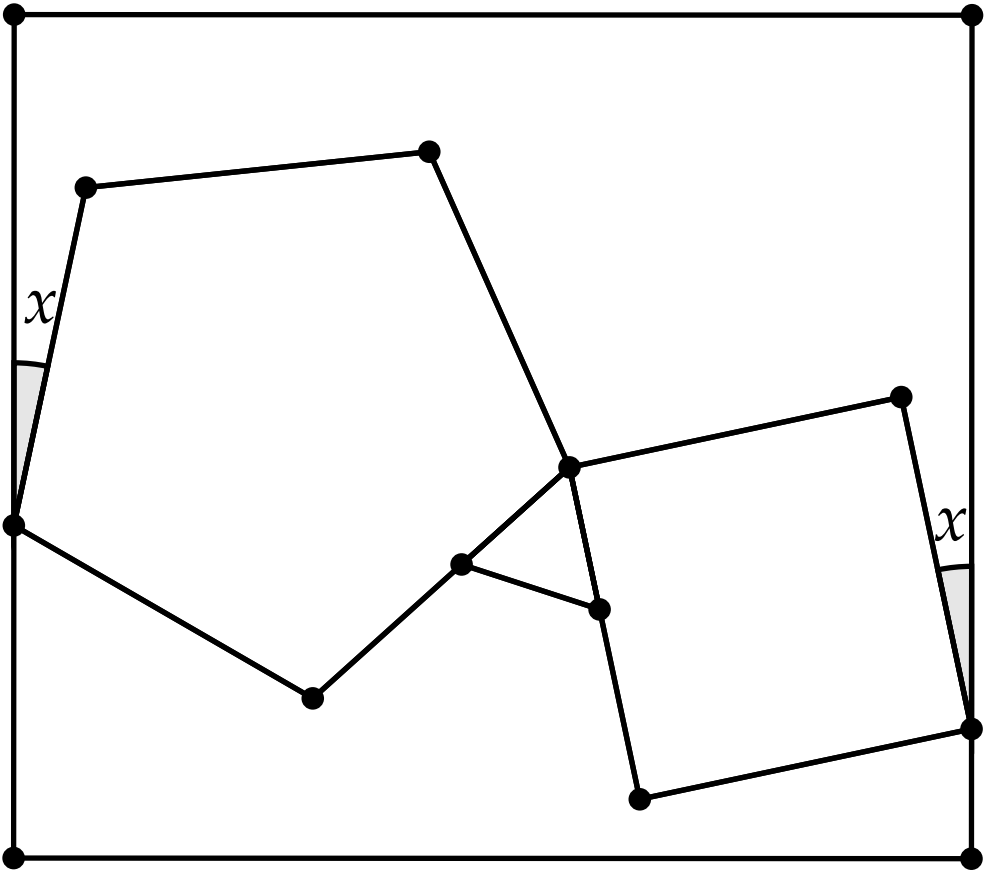
\includegraphics[width=0.4\textwidth]{second.png}
          \end{figure}

        \item Uma professora tem menos de 100 alunos e dispõe de 2024 balas para distribuí-las igualmente entre os alunos. Constatou que
          deveria comprar no mínimo 41 balas a mais para isso. Quantos alunos há na sala?
        \item Em uma cidade com 2025 habitantes, cada pessoa é mentirosa (mentem sempre) ou sincera (dizem sempre a verdade). Um dia, Ana
          diz: “Nessa cidade há um número ímpar de mentirosos!”. Com base nisso, quais das afirmações seguintes são necessariamente verdadeiras?
        \item No retângulo \(ABCD\), \(AB = 8\) e \(BC = 4\). \(E\) e \(F\) são os pontos médios de \(CD\) e \(AB\), respectivamente. A reta 
          \(AE\) intersecta \(BC\) no ponto \(G\), e a reta \(GF\) intersecta \(AD\) no ponto \(H\). Qual é a área do triângulo \(AGH\)?
          \begin{figure}[h]
            \centering
            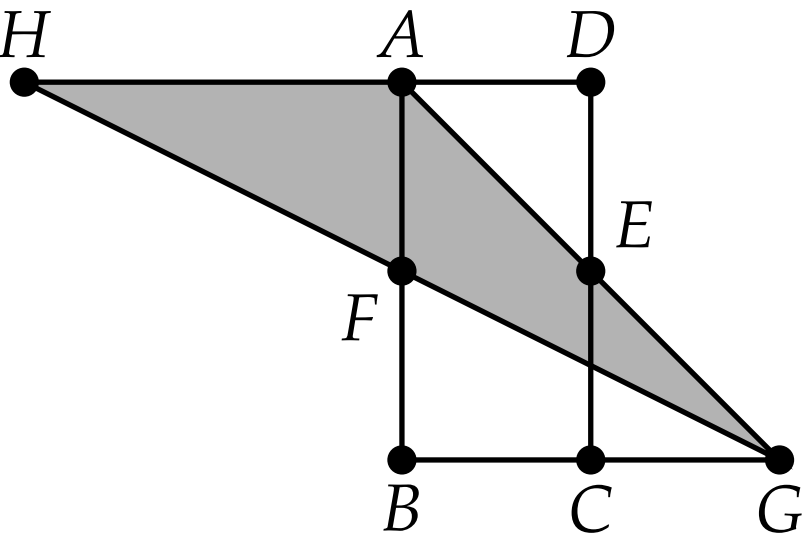
\includegraphics[width=0.4\textwidth]{third.png}
          \end{figure}
        \item No planeta Xorpzorp, as semanas têm 11 dias (1ª-feira a 11ª-feira); os meses alternam entre 50 e 51 dias; o ano tem exatamente
          5 meses, alternando entre 252 e 253 dias. Hoje é 4ª-feira, dia 51 do mês 4 de 2024. Após 24 anos terrestres, qual será a data no
          calendário de Xorpzorp?
        \item No triângulo isósceles com base \(BC\), pontos \(E\) em \(AB\) e \(F, G\) em \(AC\) satisfazem: (i) \(A, F, G, C\) estão nessa 
          ordem; (ii) \(AF = EF\); (iii) \(EF\) é bissetriz de \(\angle AEG\); (iv) \(GB\) é bissetriz de \(\angle EGC\); (v) \(BC = BG\).
          Qual é o valor de \(\angle BAC\)?
        \item Maria escreveu os primeiros 1000 múltiplos de 23, em ordem, e José apagou os dígitos de ordem a partir das centenas (por exemplo,
          12345 vira 345). Restou uma lista de 1000 números com até 3 dígitos. Qual número dessa lista aparece por último em ordem
          (entre 112, 113, 114, 115 e 116)?
        \item As circunferências \(\omega_1\), centro \(A\), passando por \(B\), e \(\omega_2\), centro \(B\), passando por \(A\), se
          intersectam em \(C\). A reta \(BC\) intersecta \(\omega_2\) novamente em \(D\). A reta \(DA\) intersecta \(\omega_1\) em \(E\)
          (com \(A\) entre \(D\) e \(E\)). A reta \(EB\) intersecta \(\omega_2\) em \(F\) (com \(B\) entre \(E\) e \(F\)). Determine 
          \(\angle DEF\) em graus.
          \begin{figure}[h]
            \centering
            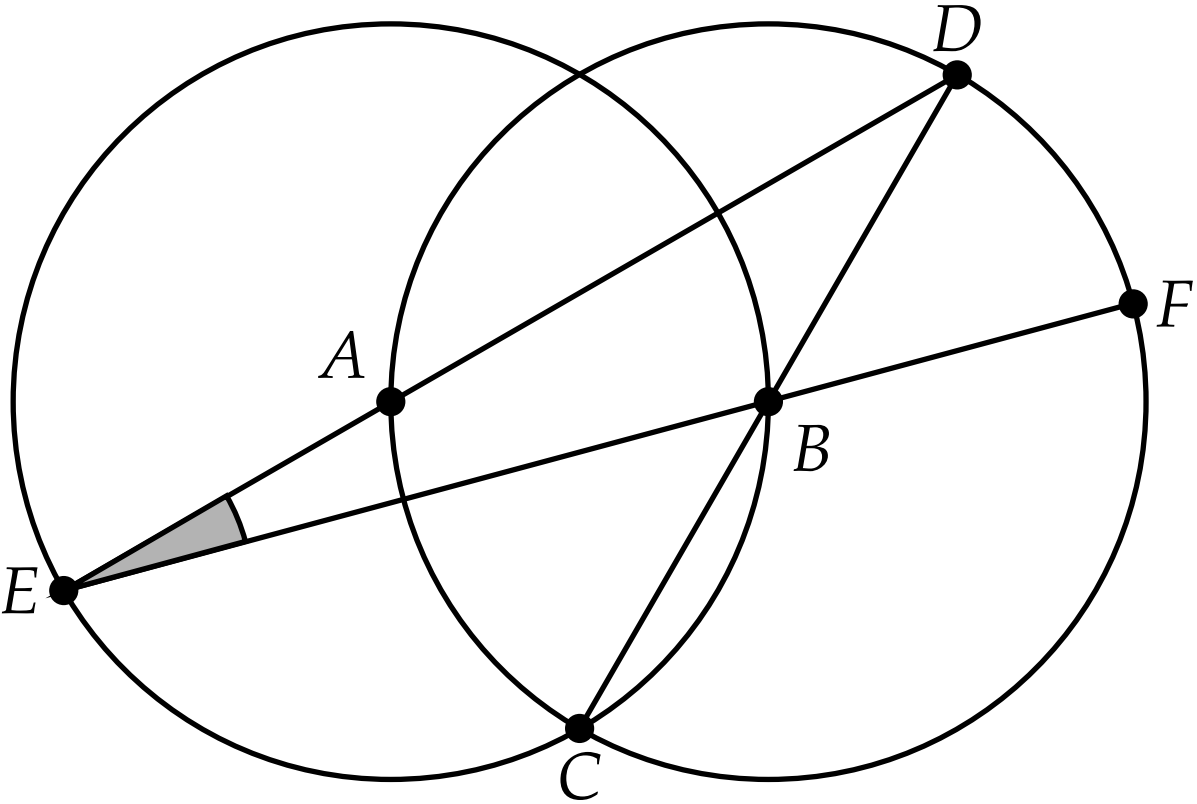
\includegraphics[width=0.5\textwidth]{fourth.png}
          \end{figure}
        \item Em uma figura, os pontos \(E, F, G, H, I, J\) devem ser pintados, um por um, com as cores vermelho, verde ou azul, de modo que
          três pontos colineares não tenham a mesma cor. Quantas pinturas possíveis existem?
          \begin{figure}[h]
            \centering
            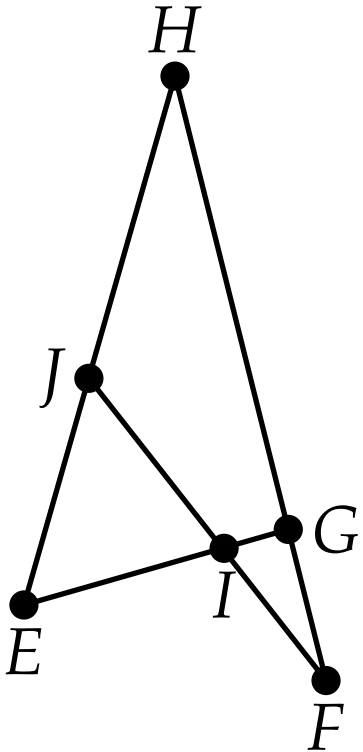
\includegraphics[width=0.15\textwidth]{fifth.png}
          \end{figure}
        \item O sistema
          \[
            \begin{cases}
              a^3 + b = 4c,\\
              a + b^3 = c,\\
              ab = -1
            \end{cases}
          \]
          tem solução real. Quantos valores de \(a\) satisfazem o sistema?
        \item Um tabuleiro \(15 \times 36\) será coberto, sem sobreposição, por quadrados de lado \(5 \times 5\) e \(7 \times 7\). Nenhuma
          parte das peças pode sair do tabuleiro. Qual é o número mínimo de quadradinhos que permanecerão descobertos?
      \end{enumerate}
    \subsection{Respostas Numéricas}
      \begin{enumerate}[label=\textbf{\arabic*.}, start=16]
        \item Seja \(N\) um inteiro positivo de quatro algarismos cujo algarismo das unidades é igual a 3 e seja \(M\) o número obtido de
          \(N\) apagando esse algarismo 3 e escrevendo-o no começo de \(N\). Sabe-se que \(M\) é 2025 unidades menor que \(N\).Qual é o valor
          de \(N\)?
        \item Um número \(a\) ganha de outro \(b\) se \(a>b\) e o número obtido invertendo os dígitos de \(a\) na base decimal é maior do que
          o número obtido invertendo os dígitos de \(b\). Por exemplo, 314 ganha de 291, pois 314>291 e 413>192. Por outro lado, 314 não ganha
          de 309, pois 413<903. Quantos números de quatro algarismos ganham de 2024?
        \item Considere a expressão
          \[
            1\ 2\ 3\ \ldots\ 2023\ 2024.
          \]
          Em cada espaço vazio, coloque um \(+\) ou um \(-\) e calcule o resultado. Quantos são os possíveis restos desse resultado na
          divisão por 2024?
        \item Sejam \(a,b,c\) tais que
          \[
            \begin{cases}
              a+b+c=10,\\
              a^2+b^2+c^2=20,\\
              a^3+b^3+c^3=30.
            \end{cases}
          \]
          Calcule o valor de \(a^5+b^5+c^5\).
        \item Na figura a seguir temos um paralelogramo em que cada lado foi dividido em três partes iguais. Os pontos sobre os lados foram
          ligados alternadamente para formar dois quadriláteros. A figura sombreada é formada pela união das regiões desses dois quadriláteros.
          A razão entre a área sombreada e a área do paralelogramo pode ser escrita como fração irredutível \(\tfrac{p}{q}\), com \(p,q\)
          inteiros positivos. Quanto vale \(p+q\)?
          \begin{figure}[h]
            \centering
            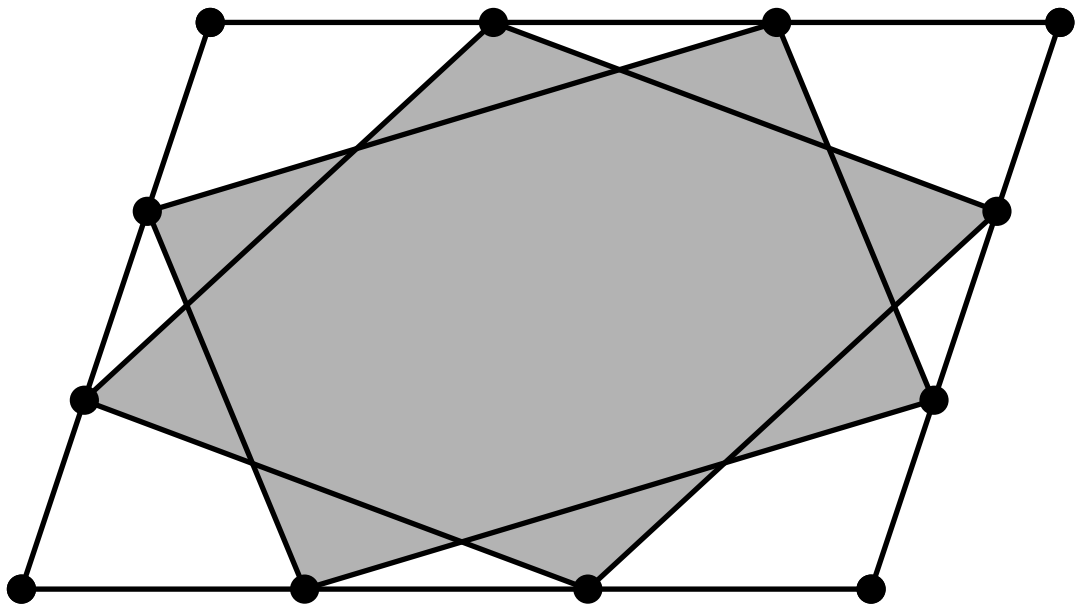
\includegraphics[width=0.4\textwidth]{sixth.png}
          \end{figure}
      \end{enumerate}
  \clearpage

  \section{\textsf{Soluções}}
    \subsection{Testes}
    \subsection{Respostas Numéricas}

  \clearpage

  \section{\textsf{Referências}}
\end{document}
